\documentclass[11pt, oneside]{article}   	% use "amsart" instead of "article" for AMSLaTeX format
\usepackage{geometry}                		% See geometry.pdf to learn the layout options. There are lots.
\geometry{letterpaper}                   		% ... or a4paper or a5paper or ... 
%\geometry{landscape}                		% Activate for rotated page geometry
%\usepackage[parfill]{parskip}    		% Activate to begin paragraphs with an empty line rather than an indent
\usepackage{graphicx}				% Use pdf, png, jpg, or eps§ with pdflatex; use eps in DVI mode
								% TeX will automatically convert eps --> pdf in pdflatex
\usepackage{tikz}
\usetikzlibrary{positioning,arrows,quotes, shapes}
\tikzset{m/.style={circle,draw,fill=gray!40,minimum size=20},
            b/.style={ellipse,draw,fill=gray!40,minimum size=20}, outer sep=5pt}
\usepackage{siunitx}

\usepackage{amssymb}

%SetFonts

%SetFonts


\title{Nonparametric Bayesian analysis using Normalizing Flows (better funner title, please)}
\author{Ji, Jiang, Tan, Wang, Schwartz}
%\date{}							% Activate to display a given date or no date

\begin{document}
\maketitle

\section{Introduction}

All explanations should be about one to two sentences only, and should primarily rely upon appropriate referencing.

\subsection{Bayesian Analysis (Haining/Yichen)}
\begin{itemize}
\item Bayesian updating, including posteriors as subsequent priors
\item General arguments: full uncertainty characterization, Bayesian model averaging [Yichen]
\item General criticisms: priors [Yichen]
\item MCMC/MH/HMC
\item VI
\item Importance Sampling
\end{itemize}

\subsection{Bayesian Deep Learning (Yichen/Eric/Haining)}
\begin{itemize}
\item General criticisms
\item BBB
\item GP approximation with MC-dropout [Eric]
\item SWAG
\item criticize VAE "bayesian language" usage (to clarify what of focus is in Bayesian analysis) [Haining] 
\end{itemize}

\subsection{Normalizing Flows (Ryan/Yichen)}
\begin{itemize}
\item Introduction to Generative Models [Yichen]
\item Conditioners
\item Transformer/Coupling functions
\item Alternatives such as stochastic ODEs
\item Computation
\item Importance sampling under base-to-target as prior-to-posterior (e.g., SNF, Müller)
\end{itemize}

\section{Method (Scott first draft)}

The sequential nature of Bayesian learning $p(\theta | x_1,x_2) \propto p(\theta)f(x_1|\theta) f(x_2|\theta) \propto q(\theta) f(x_2|\theta)$ for data partition $x=(x_1,x_2)$ allows a composite analysis based on incorporating $x_1$ into an intermediate prior $q(\theta) \propto p(\theta) f(x_1 | \theta )$. 
For some intermediate prior approximation $q_\phi(\theta) \approx p(\theta |x_1)$ as the proposal distribution for the target distribution $q(\theta|x_2) = p(\theta | x_1,x_2)$, the target to proposal densities ratio defining (unnormalized) importance sampling weights \cite{BayesIS} are

$$w(\theta) \propto \frac{q(\theta|x_2)}{q_\phi(\theta)} \propto \frac{f(x_2| \theta) f(x_1| \theta) p(\theta) }{q_\phi(\theta)}  \propto \frac{f(x_2| \theta) q(\theta) }{q_\phi(\theta)}  \approx  f(x_2| \theta)$$

\noindent where the approximation is accurate insofar as the cancellation holds.  For $\theta \in I \!\! R^d$ for large $d$, using a proposal distribution $q_\phi(\theta)$ which approximates the (intermediate prior) partial posterior $p(\theta |x_1)$ facilitates efficient importance sampling by targeting proposals around $E[\theta | x_1] \approx E[\theta | x]$ and balancing importance weights 
$w(\theta^{(k)})  \approx  f(x_2| \theta^{(k)}) /  \sum_j f(x_2| \theta^{(j)})$ 
by controlling posterior concentration to bound relative tail ratios $\frac{q(\theta|  x_2)}{q_\phi(\theta)} \approx f(x_2| \theta )< c$.

The approximation of the partial posterior $q_\phi(\theta) \approx p(\theta |x_1)$ is produced by SWAG \cite{SWAG19} for the data model $f(x_1| \theta)$, the $x_1$ subset of $x$, and the unupdated prior $p(\theta)$. Samples from this intermediate prior approximation are then (approximately) representative of the full posterior $p(\theta | x_1,x_2) = q(\theta | x_2)$ in proportion to the likelihood approximation of their (unnormalized) importance weights $w(\theta)$ computed from the data model $f(x_2| \theta)$,  the $x_2$ subset of $x$, and the sample from $q_\phi(\theta)$.  The data model itself can be flexibly estimated through a likelihood-defining neural network (NN) such as a normalizing flow (NF) \cite{NFreview} defining $f(x|\theta) = f(z=g^{-1}_{\theta_0}\circ \cdots \circ g^{-1}_{\theta_T}(x)) \prod_{t=0}^T | \det J_{g^{-1}_{\theta_t}}(x) |$. Thus, $p(\theta | x)$ characterizes posterior uncertainty in the data model $f(x|\theta)$ given data $x$.

Importantly, as illustrated in Figure \ref{fig1}, the NF defines the likelihood $f(x|\theta)$ upon which the SWAG approximation of a (intermediate prior) partial posterior is based, and also defines the approximation of importance sampling weights $w(\theta)$ for posterior importance sampling based on $q_\phi(\theta)$. This is different than interpreting a NF as transforming a `prior' base distribution into a posterior target distribution in order to transform samples from the `prior' into (potentially importance sampling reweighted) samples from the posterior \ref{basepriortargetposteriorIS}.  While this latter computation is implicitly Bayesian based on its assumption of an externally derived posterior target, the approach presented here is explicitly Bayesian in defining a likelihood and providing Bayesian updates on the parameters $\theta$ of the likelihood given the available data. 

\begin{figure}
\centering
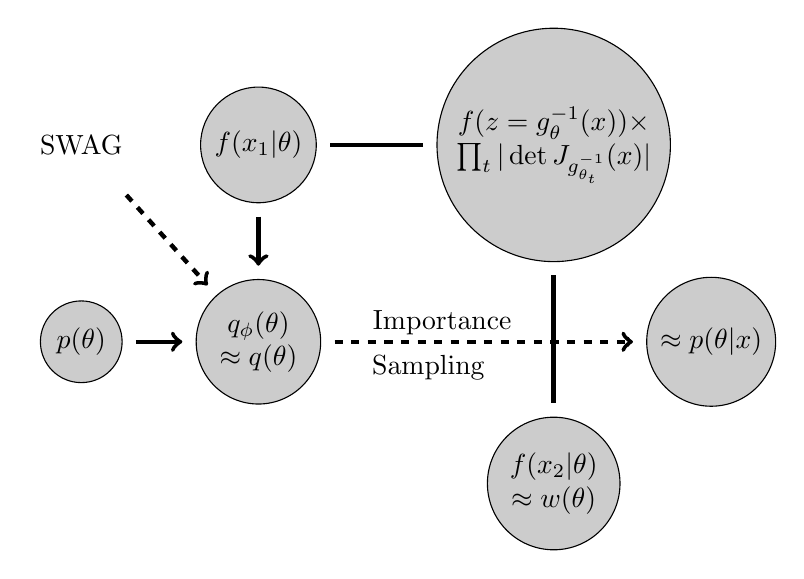
\begin{tikzpicture}
\node[circle] at (0,2.5)(0){SWAG};
\node[m] at (-0,0)(1){$p(\theta)$};
\node[m] at (2.25,2.5)(2){$f(x_1|\theta)$};
\node[m, align=center] at (2.25,0)(3){$q_\phi(\theta)$\\$\approx q(\theta)$};
\node[m, align=center] at (6,2.5)(4){$f(z=g^{-1}_\theta(x)) \times$\\$\prod_t | \det J_{g^{-1}_{\theta_t}}(x) |$};
\node[m] at (8, 0)(5){$\approx p(\theta|x)$};
\node[m, align=center] at (6,-1.8)(6){$f(x_2|\theta)$\\$\approx w(\theta)$};
\draw[->, dashed, ultra thick] (0) edge (3);
\draw[->, ultra thick] (1) edge (3);
\draw[->, ultra thick] (2) edge (3);
\draw[->, dashed] (3) edge ["Importance$\quad\quad\quad$" {yshift=-6pt} ] (5); 
\draw[->, dashed, ultra thick] (3) edge ["Sampling$\quad\quad\quad\quad$" {yshift=-22pt} ] (5); 
\draw[-, ultra thick] (4) edge (2);
\draw[-, ultra thick] (4) edge (6);
\end{tikzpicture}
\caption{A visual representation of the components of the methodology. The dashed arrows indicated Bayesian posterior sampling methodologies.  SWAG approximates the usual posterior derivation indicated by the solid arrows, and importance sampling reweights samples from the (intermediate) prior distribution by their likelihood values to produce a representation of the posterior. The $x_1$ and $x_2$ indicate that this occurs sequentially, and the solid lines indicate the use of the (same) data model $f(x|\theta)$ in both posterior derivations. If the SWAG approximation of $q(\theta)$ is solely viewed as a proposal distribution, then the importance weight $w(\theta)$ can be computed exactly, and the posterior approximation is exact. This characterizes posterior uncertainty over the parameters $\theta$ of the data model $f(x|\theta)$.}
\end{figure}

The approximation $q_\phi(\theta) \approx q(\theta)$ can be pragmatically viewed as a prior specification.  This entails some ``misuse" of the $x_1$ posterior update relative to $p(\theta)$, but can nonetheless be viewed as a practical ``empirical Bayes'' \ref{empiricalBayes} method for prior elicitation \ref{priorElicitation}. If taken as a prior, the importance sampling weights $w(\theta) = f(x_2|\theta)$ are exact relative to $q_\phi(\theta)$ for the altered posterior $q_\phi(\theta|x_2) \approx p(\theta|x)$, where the approximation improves the larger the $x_2$ subset of $x$ is. 
Alternatively, the importance sampling weights $w(\theta) = \frac{f(x|\theta)p(\theta)}{q_\phi(\theta)}$ are exact relative to $q(\theta)$ for the original posterior $q(\theta|x_2) = p(\theta|x)$ as will remain relatively balanced so long as $p(\theta)$ is relatively heavy-tailed. 

While focus may be on $p(\theta|x)$ explicitly as in ``Bayes by backprop" \ref{BBB}, more generally interest is in $p\left(h(\theta) | x \right)$.   For example, ``MC-dropout'' \ref{MCdropout} approximates a Gaussian process posterior and so is interested in $p\left( f_\theta | x \right)$.  Similarly, the NF likelihood $f_{x_0}(\theta) = f(x_0 | \theta) $ evaluated at $x_0$ has the posterior distribution  $p\left( f_{x_0}(\theta) | x \right)$ which propagates and aggregates the uncertainty in $p(\theta|x)$.
So just as the posterior CDF $F_{\theta|x}$ can be estimated using importance samples representing $p(\theta|x)$, so too can the CDF $F_{f(x_0 | \theta)|x}$; namely, for importance samples $\theta_i$ and corresponding weights $w(\theta_i)$, $F_{f(x_0 | \theta)|x}(\theta) = \sum_{i=1}^n w(\theta_i) 1_{[F_{f(x_0 | \theta)|x}(\theta) \leq F_{f(x_0 | \theta_i)|x}(\theta_i)]}$.







\subsection{nonparametric NF likelihood, SWAG prior, importance sampling posterior}
\subsection{computation: core sets, online covariance estimation, sampling}

\section{Examples}
\subsection{mean variance normal posterior}
\subsection{repeat SWAG analyses}
\subsection{regression}
\subsection{mixed effects models}

\section{Discussion}

\end{document}  


\begin{figure}
\centering
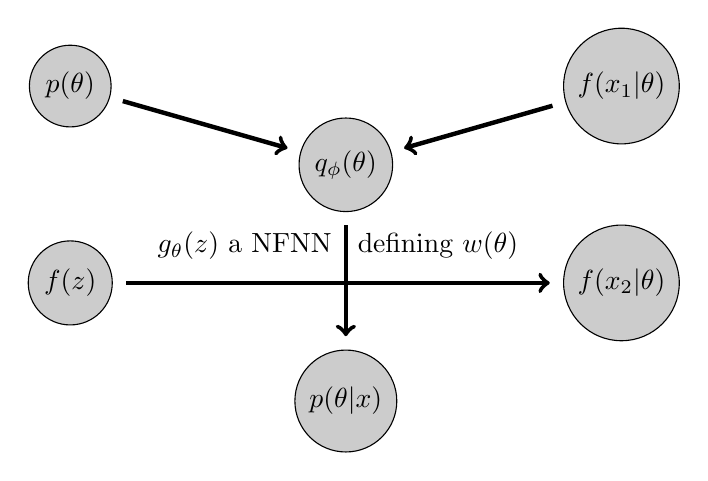
\begin{tikzpicture}
\node[m] at (0,0)(1){$f(z)$};
\node[m] at(7,0)(2){$f(x_2|\theta)$};
\node[m] at(3.5, 1.5)(3){$q_\phi(\theta)$};
\node[m] at(3.5, -1.5)(4){$p(\theta|x)$};
\node[m] at (0,2.5)(5){$p(\theta)$};
\node[m] at (7,2.5)(6){$f(x_1|\theta)$};
\draw[->, ultra thick] (1) edge ["$g_\theta(z)$ a NFNN $\;$ defining $w(\theta)$"] (2);
\draw[->, ultra thick] (3) edge (4);
\draw[->, ultra thick] (5) edge (3);
\draw[->, ultra thick] (6) edge (3);
\end{tikzpicture}
\label{fig1}
\end{figure}

